\documentclass[tikz,border=10pt]{standalone}
\usetikzlibrary{shapes, arrows.meta, positioning, calc}

\begin{document}
	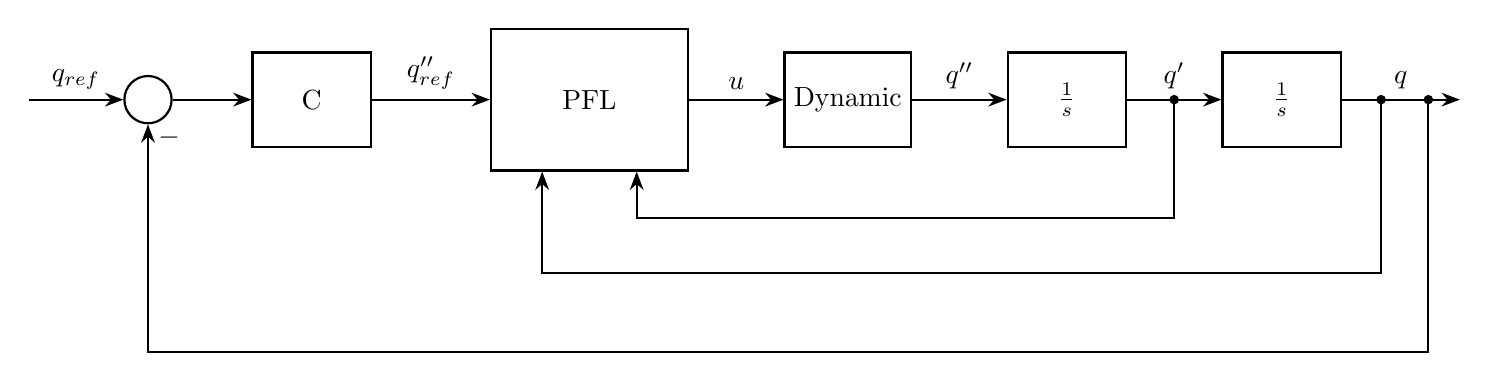
\begin{tikzpicture}[
		>=Stealth,
		auto,
		node distance=1.5cm,
		% Estilos de los bloques
		block/.style={draw, rectangle, thick, minimum height=1.2cm, minimum width=1.5cm, align=center, fill=white},
		sum/.style={draw, circle, thick, inner sep=2pt, minimum size=0.6cm},
		line/.style={draw, thick, ->}
		]
		
		% --- NODOS (BLOQUES) ---
		
		% Entrada y sumador
		\coordinate (input) at (0,0);
		\node [sum, right=1.2cm of input] (sum) {};
		
		% Bloques principales
		\node [block, right=1cm of sum] (C) {C};
		\node [block, right=1.5cm of C, minimum width=2.5cm, minimum height=1.8cm] (PFL) {PFL};
		\node [block, right=1.2cm of PFL] (dynamic) {Dynamic};
		\node [block, right=1.2cm of dynamic] (int1) {$\frac{1}{s}$};
		\node [block, right=1.2cm of int1] (int2) {$\frac{1}{s}$};
		
		% --- LÍNEAS DIRECTAS (FORWARD PATH) ---
		\draw [line] (input) -- node {$q_{ref}$} (sum);
		\draw [line] (sum) -- (C);
		\draw [line] (C) -- node {$q_{ref}''$} (PFL);
		\draw [line] (PFL) -- node {$u$} (dynamic);
		\draw [line] (dynamic) -- node {$q''$} (int1);
		\draw [line] (int1) -- node [name=qdot] {$q'$} (int2);
		
		% Salida final
		\coordinate (output) at ($(int2.east) + (1.5,0)$);
		\draw [line] (int2) -- node [name=q] {$q$} (output);
		
		% --- LAZOS DE REALIMENTACIÓN (FEEDBACK) ---
		
		% 1. Feedback de q' al PFL
		\coordinate (fb1) at ($(int1.east) + (0.6,0)$);
		\filldraw (fb1) circle (1.5pt); % Punto de conexión
		\draw [line] (fb1) -- ++(0,-1.5) -| ($(PFL.south) + (0.6,0)$);
		
		% 2. Feedback de q al PFL
		\coordinate (fb2) at ($(int2.east) + (0.5,0)$);
		\filldraw (fb2) circle (1.5pt); % Punto de conexión
		\draw [line] (fb2) -- ++(0,-2.2) -| ($(PFL.south) + (-0.6,0)$);
		
		% 3. Feedback principal (q al sumador)
		\coordinate (fb3) at ($(int2.east) + (1.1,0)$);
		\filldraw (fb3) circle (1.5pt); % Punto de conexión
		\draw [line] (fb3) -- ++(0,-3.2) -| node [pos=0.97, right] {$-$} (sum.south);
		
	\end{tikzpicture}
\end{document}